\documentclass[12pt]{article}
\usepackage[utf8]{inputenc}
\usepackage[es]{babel}
\usepackage{amsmath}
\usepackage{amsfonts}
\usepackage{amssymb}
\usepackage{graphicx} 
\usepackage{booktabs}
\usepackage{float} 
\usepackage{hyperref} 
\usepackage{longtable}
\usepackage{caption}
\usepackage{subcaption}
\usepackage[margin=1in]{geometry}

\title{Análisis de Resultados y Modelo Matemático para Diseño Óptimo de Red de Distribución de Agua}
\author{Javier Sola, Martín Caballero, Bastián Jiménez, Agustín Venegas \\ \small Grupo 6}
\date{\today} 

\begin{document}

\maketitle

\begin{abstract}
Este documento presenta el análisis de los resultados obtenidos del modelo matemático de optimización para el diseño de una red de tuberías de abastecimiento de agua. Se detallan los conjuntos, parámetros, variables, función objetivo y restricciones del modelo. Además, se describe el proceso de generación de instancias de diferentes tamaños y se analiza el comportamiento de la función objetivo, la factibilidad y los tiempos de resolución utilizando el software de optimización asignado.
\end{abstract}

\clearpage
\tableofcontents
\clearpage

\section{Parte 1: Formulación del Modelo Matemático}

\subsection*{1. Conjuntos}

\begin{itemize}
  \item \( \mathcal{N} \): conjunto de todos los nodos, con \(|\mathcal{N}| = N\)
  \begin{itemize}
    \item \( \mathcal{P} \subset \mathcal{N} \): nodos plantas de tratamiento
    \item \( \mathcal{T} \subset \mathcal{N} \): nodos tanques
    \item \( \mathcal{C}_t \subset \mathcal{N} \): nodos clientes de transbordo
    \item \( \mathcal{C}_f \subset \mathcal{N} \): nodos clientes finales
  \end{itemize}
  \item \( \mathcal{A} \subseteq \mathcal{N} \times \mathcal{N} \): conjunto de arcos posibles (únicamente entre columnas adyacentes), con \(|\mathcal{A}| = A\)
  \item \( \mathcal{D} = \{1,3,4\} \): conjunto de diámetros permitidos para tuberías, con \(|\mathcal{D}| = D\)
  \item \( \mathcal{K} = \{a,b\} \): tipos de costos de instalación, con \(|\mathcal{K}| = K\)
\end{itemize}

\subsection*{2. Parámetros}

\begin{itemize}
  \item \( \text{Cap}_d \): capacidad máxima de flujo para diámetro \( d \in \mathcal{D} \) [l/min]
  \[
  \text{Cap}_1 = 353, \quad \text{Cap}_3 = 1414, \quad \text{Cap}_4 = 2036
  \]
  
  \item \( \text{Cost}_{dk} \): costo de instalación para diámetro \( d \) y tipo \( k \in \mathcal{K} \), según la tabla siguiente:
  \[
  \begin{array}{c|cc}
  \toprule
  \text{Diámetro} & \text{Costo tipo } a & \text{Costo tipo } b \\
  \midrule
  1 \quad (50\,mm) & 16 & 45 \\
  3 \quad (100\,mm) & 24 & 62 \\
  4 \quad (120\,mm) & 27 & 68 \\
  \bottomrule
  \end{array}
  \]

  \item \( c_{ij} \), para \( i=1,\ldots,N \), \( j=1,\ldots,N \): costo de transporte por unidad de flujo entre nodo \( i \) y nodo \( j \)
  \item \( d_j \), para \( j \in \mathcal{C}_f \): demanda de agua en nodo cliente final \( j \)
  \item \( S_i \), para \( i \in \mathcal{P} \): capacidad de suministro en planta \( i \)
\end{itemize}

\subsection*{3. Variables de Decisión}

\begin{itemize}
  \item \( x_{ij}^d \in \{0,1\} \), para \( i=1,\ldots,N \), \( j=1,\ldots,N \), \( d=1,\ldots,D \): variable binaria que indica si se instala tubería de diámetro \( d \) en arco \( (i,j) \)
  \[
  x_{ij}^d = \begin{cases}
  1 & \text{si se instala tubería de diámetro } d \text{ en arco } (i,j), \\
  0 & \text{en caso contrario}.
  \end{cases}
  \]

  \item \( f_{ij} \geq 0 \), para \( i=1,\ldots,N \), \( j=1,\ldots,N \): flujo de agua que circula por el arco \( (i,j) \)
\end{itemize}

\subsection*{4. Función Objetivo}

Minimizar el costo total de la red, que incluye costos de instalación y transporte:

\[
\min \sum_{i=1}^{N} \sum_{j=1}^{N} \sum_{d=1}^{D} \sum_{k=1}^{K} \text{Cost}_{dk} \cdot x_{ijd} + \sum_{i=1}^{N} \sum_{j=1}^{N} c_{ij} \cdot f_{ij}
\]

\subsection*{5. Restricciones}

\begin{enumerate}
  \item \textbf{Capacidad máxima por tubería:}
  \[
  f_{ij} \leq \sum_{d=1}^{D} \text{Cap}_d \cdot x_{ij}^d, \quad \forall i=1,\ldots,N, \quad j=1,\ldots,N
  \]

  \item \textbf{Una única tubería por arco:}
  \[
  \sum_{d=1}^{D} x_{ij}^d \leq 1, \quad \forall i=1,\ldots,N, \quad j=1,\ldots,N
  \]

  \item \textbf{Conservación de flujo (balance nodal):}
  \begin{itemize}
    \item Para tanques y nodos clientes de transbordo \( i \in \mathcal{T} \cup \mathcal{C}_t \):
    \[
    \sum_{j=1}^{N} f_{ji} = \sum_{j=1}^{N} f_{ij}
    \]
    \item Para plantas \( i \in \mathcal{P} \):
    \[
    \sum_{j=1}^{N} f_{ij} \leq S_i
    \]
    \item Para nodos clientes finales \( i \in \mathcal{C}_f \):
    \[
    \sum_{j=1}^{N} f_{ji} = d_i
    \]
  \end{itemize}

  \item \textbf{Restricción de conectividad:} solo se permiten arcos entre columnas adyacentes:
  \[
  \mathcal{P} \to \mathcal{T}, \quad \mathcal{T} \to \mathcal{C}_t, \quad \mathcal{C}_t \to \mathcal{C}_f
  \]

  \item \textbf{Dominio y no negatividad:}
  \[
  x_{ij}^d \in \{0,1\}, \quad f_{ij} \geq 0, \quad \forall i=1,\ldots,N, \quad j=1,\ldots,N, \quad d=1,\ldots,D
  \]
\end{enumerate}

\subsection{Generación de Instancias}

Para validar el modelo matemático, se generaron instancias clasificadas en tres tamaños: pequeño, mediano y grande. Los rangos para la cantidad de nodos de cada tipo se muestran en la Tabla~\ref{tab:rangos_nodos}.

\begin{table}[h]
\centering
\caption{Rangos para generación de nodos según tamaño de instancia}
\label{tab:rangos_nodos}
\begin{tabular}{|l|c|c|c|c|}
\hline
\textbf{Tamaño} & \textbf{Plantas} & \textbf{Tanques} & \textbf{Clientes Transbordo} & \textbf{Clientes Finales} \\
\hline
Pequeño & 1--2 & 5--10 & 5--10 & 10--20 \\
\hline
Mediano & 3--4 & 10--20 & 10--20 & 20--50 \\
\hline
Grande & 5--7 & 20--50 & 25--50 & 50--100 \\
\hline
\end{tabular}
\end{table}

El proceso de generación de cada instancia consiste en:

\begin{itemize}
    \item Selección aleatoria de la cantidad de nodos para cada tipo, dentro de los rangos definidos para el tamaño de la instancia, utilizando una semilla fija para asegurar reproducibilidad.
    \item Creación de nodos identificados de forma única para plantas, tanques, clientes de transbordo y clientes finales.
    \item Construcción de la red de conexiones (arcos) entre nodos de columnas adyacentes, generando arcos de plantas a tanques, tanques a clientes de transbordo y clientes de transbordo a clientes finales.
    \item Generación de demandas para los clientes finales mediante una distribución uniforme \(U(40,100)\) litros por minuto.
    \item Asignación de costos de transporte por arco generados con distribución normal \(N(8, 2)\), truncando valores menores a 1 para evitar costos irrealmente bajos.
    \item Distribución equitativa del suministro total requerido entre las plantas generadas.
\end{itemize}

Este método permite obtener instancias variadas y reproducibles para evaluar el comportamiento del modelo.

\subsubsection{Condiciones de Factibilidad}

Para asegurar que el modelo sea factible, se consideran las siguientes condiciones:

\begin{enumerate}
    \item \textbf{Capacidad total de suministro:} La suma de las capacidades asignadas a las plantas debe ser al menos igual a la suma total de demandas de los clientes finales:
    \[
    \sum_{i \in \mathcal{P}} S_i \geq \sum_{j \in \mathcal{C}_f} d_j
    \]
    Esto garantiza que el agua demandada pueda ser suministrada desde las plantas sin exceder su capacidad máxima.
    
    \item \textbf{Capacidades máximas de tuberías:} El flujo en cada arco debe respetar la capacidad máxima determinada por el diámetro de la tubería instalada:
    \[
    f_{ij} \leq \max_{d \in \mathcal{D}} \text{Cap}_d, \quad \forall (i,j) \in \mathcal{A}
    \]
    Esta restricción asegura que el flujo no sobrepase la capacidad hidráulica del tramo instalado.
    
    \item \textbf{Costos positivos y definidos:} Los costos de instalación y transporte deben ser siempre positivos y definidos, evitando soluciones triviales o no realistas.
    
    \item \textbf{Restricción de conectividad:} La red debe respetar la estructura de conexión entre columnas adyacentes:
    \[
    \mathcal{P} \rightarrow \mathcal{T}, \quad \mathcal{T} \rightarrow \mathcal{C}_t, \quad \mathcal{C}_t \rightarrow \mathcal{C}_f
    \]
    Esto mantiene la coherencia hidráulica y estructural del sistema.
\end{enumerate}

El código generador de instancias puede ser consultado en el buzón del aula. Además, se encuentra disponible en el siguiente repositorio para su visualización y descarga: \url{https://github.com/RepublicaDePirque/Codigo-Proyecto-opti.git}.


\clearpage
\section{Parte 2: Análisis de Resultados}

\subsection{Software Asignado}
El Grupo 6 ha sido asignado para utilizar el software \textbf{LPSolve}.

LPSolve es un solucionador de programas lineales y enteros mixtos de código abierto. La implementación del modelo matemático se realiza mediante la generación de archivos con formato `.lp`, los cuales son interpretados y resueltos por LPSolve. Este enfoque permite la validación del modelo formulado y el análisis de los resultados obtenidos.

\subsection{Análisis de Resultados}
En esta sección, se presenta el análisis de los resultados de la ejecución del modelo de optimización sobre las instancias generadas.

\subsubsection{Análisis de la Función Objetivo}
Se generaron y resolvieron 6 instancias (2 pequeñas, 2 medianas y 2 grandes) utilizando LPSolve. La función objetivo representa el costo total minimizado de la red, incluyendo costos de instalación y transporte.

\begin{table}[H]
    \centering
    \caption{Resultados de la Función Objetivo por Tamaño de Instancia}
    \label{tab:FO_resultados}
    \begin{tabular}{|c|c|c|}
        \hline
        \textbf{Instancia} & \textbf{Tamaño} & \textbf{Costo Total (Función Objetivo)} \\
        \hline
        Instancia 1 & Small & 30834,0474040404 \\
        Instancia 2 & Small & 31478,3084141414 \\
        \hline
        Instancia 1 & Medium & 60047,046967676 \\
        Instancia 2 & Medium & 72467,5619979798 \\
        \hline
        Instancia 1 & Large & 284893,537482828 \\
        Instancia 2 & Large & 333093,001845455 \\
        \hline
    \end{tabular}
\end{table}

\begin{figure}[H]
    \centering
    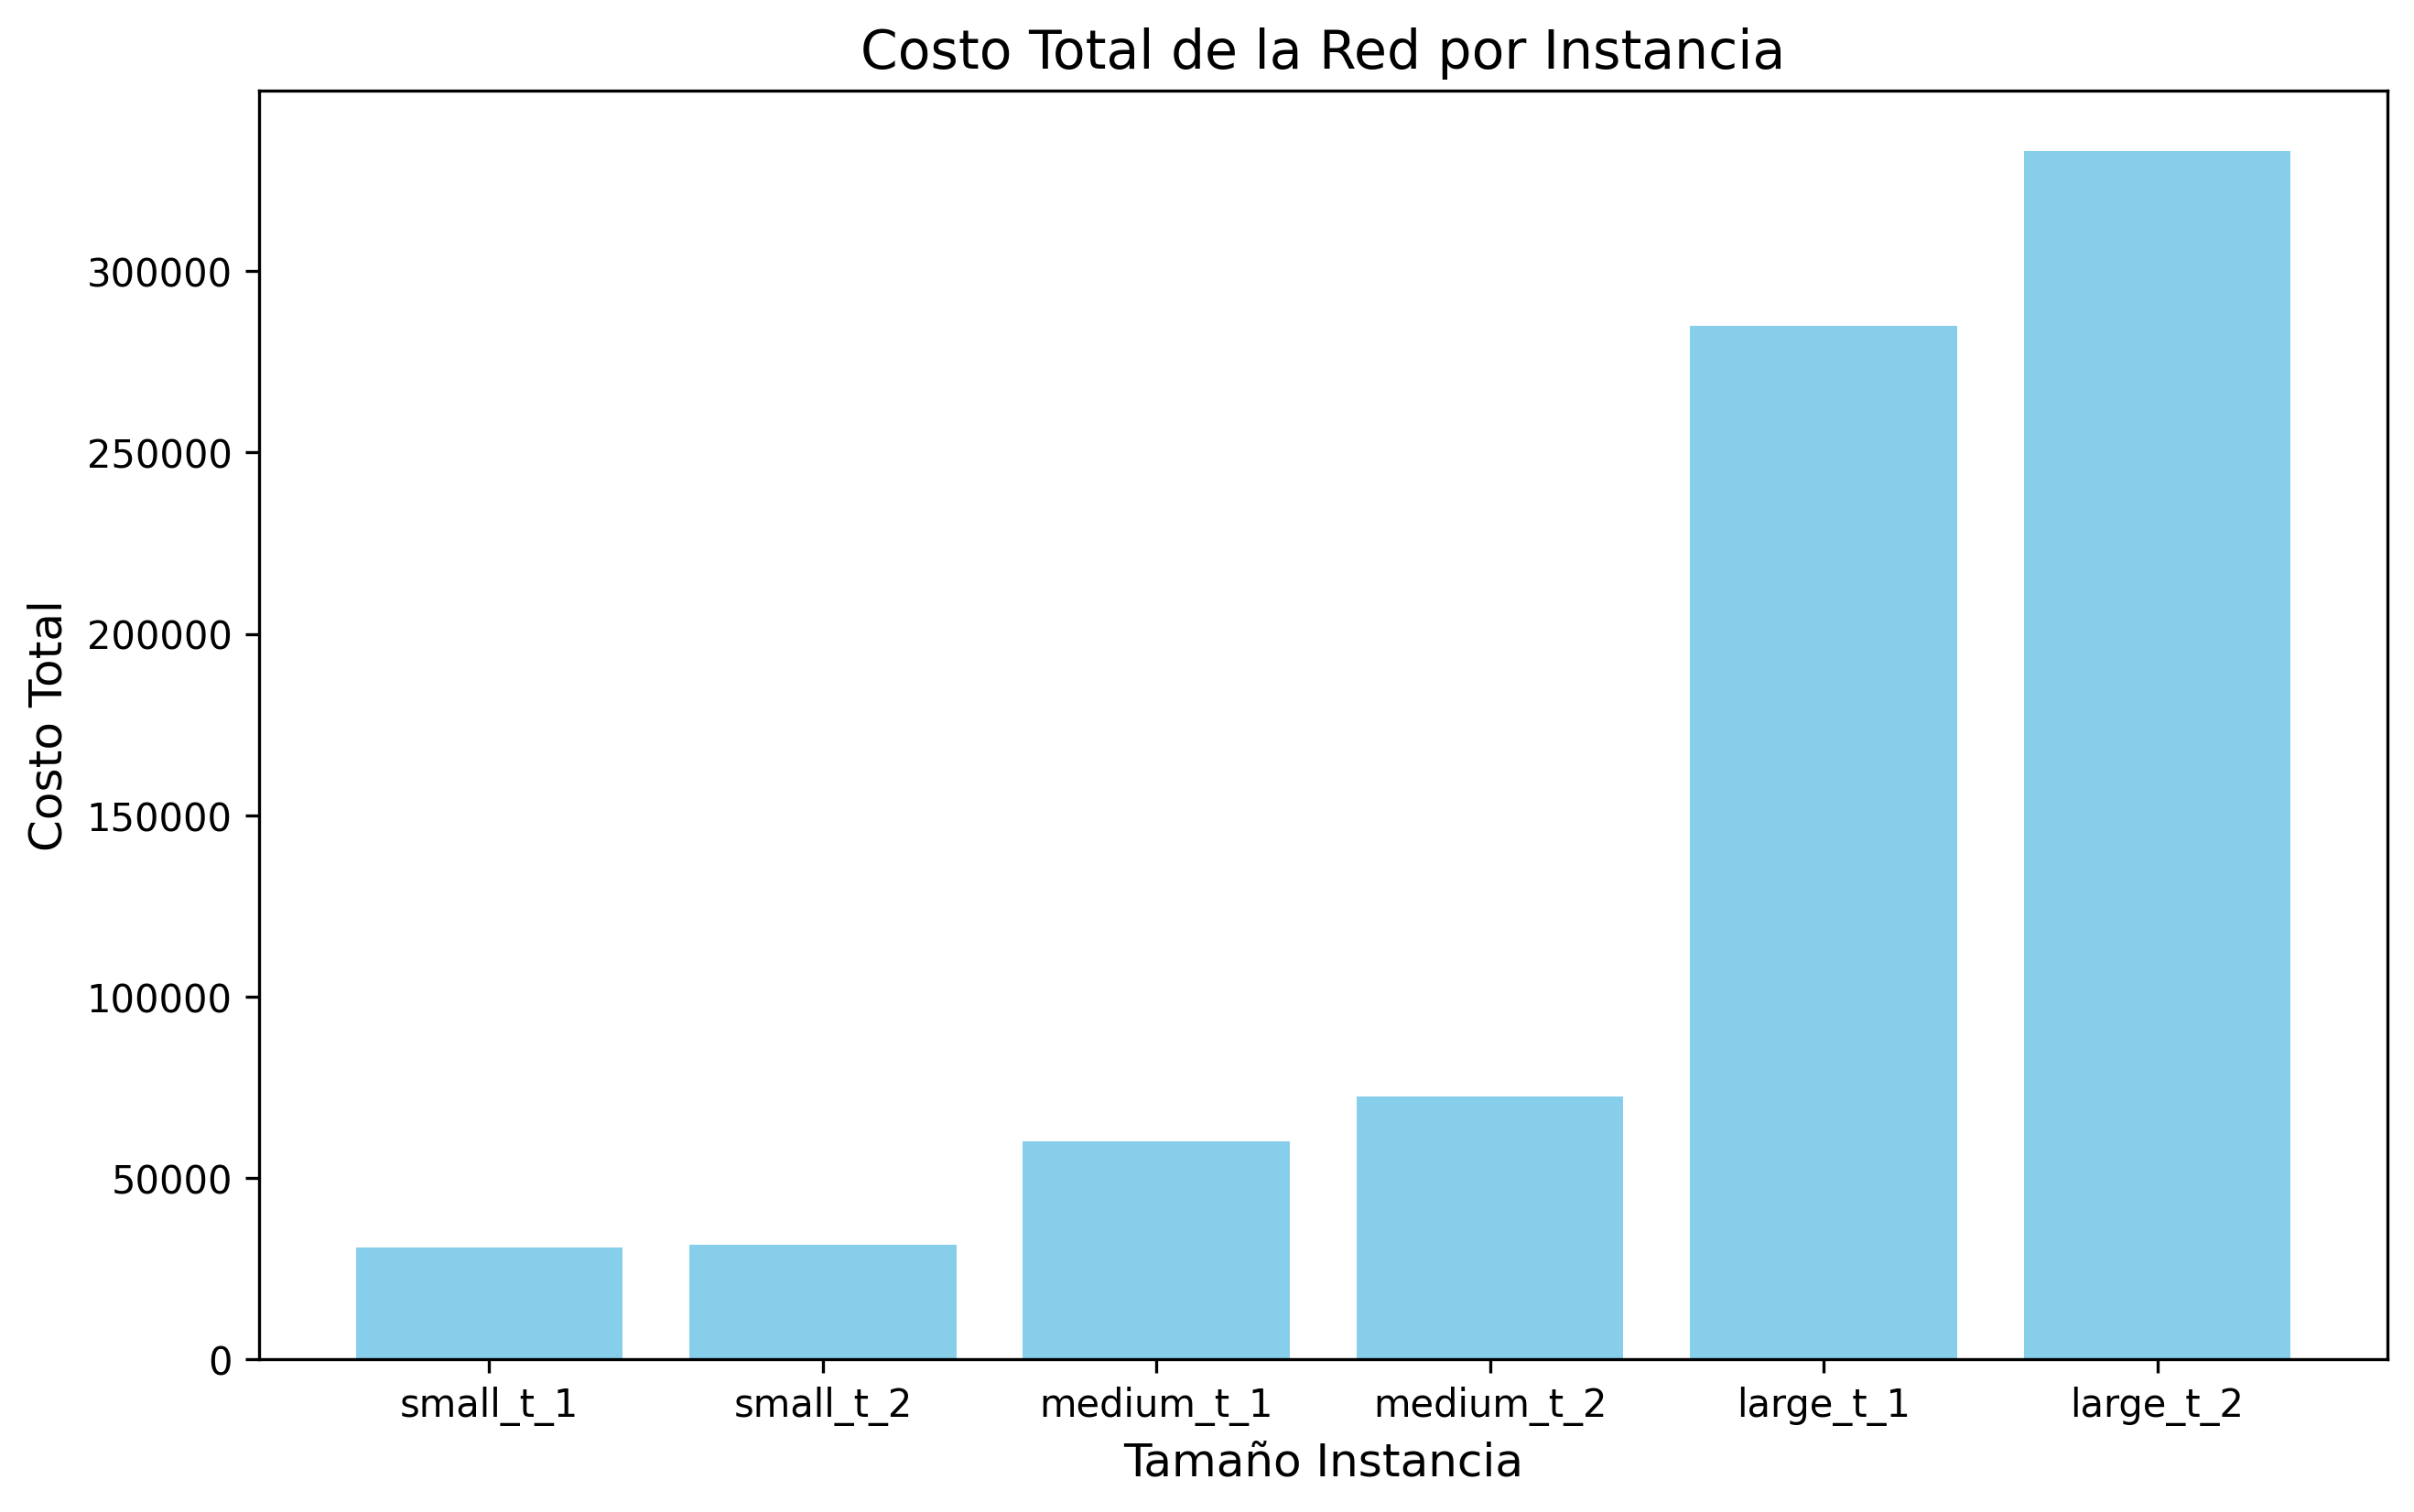
\includegraphics[width=0.8\textwidth]{of_values.png}
    \caption{Comportamiento de la Función Objetivo vs. Tamaño de la Instancia}
    \label{fig:FO_comportamiento}
\end{figure}

\subsubsection{Análisis de Factibilidad}
La factibilidad de un problema de optimización indica si existe al menos una solución que satisfaga todas las restricciones. En todas las instancias probadas, las soluciones fueron factibles y óptimas.

\subsection{Análisis de Tiempos de Resolución}
Se analizó el tiempo que LPSolve tarda en encontrar la solución óptima para las diferentes instancias.

\begin{table}[H]
    \centering
    \caption{Tiempos de Resolución por Tamaño de Instancia}
    \label{tab:Tiempos_resolucion}
    \begin{tabular}{|c|c|c|}
        \hline
        \textbf{Instancia} & \textbf{Tamaño} & \textbf{Tiempo de Resolución [segundos]} \\
        \hline
        Instancia 1 & Small & 0.014 \\
        Instancia 2 & Small & 0.013 \\
        \hline
        Instancia 1 & Medium & 0.072 \\
        Instancia 2 & Medium & 1.728 \\
        \hline
        Instancia 1 & Large & 3.028 \\
        Instancia 2 & Large & 4.228 \\
        \hline
    \end{tabular}
\end{table}

\begin{figure}[H]
    \centering
    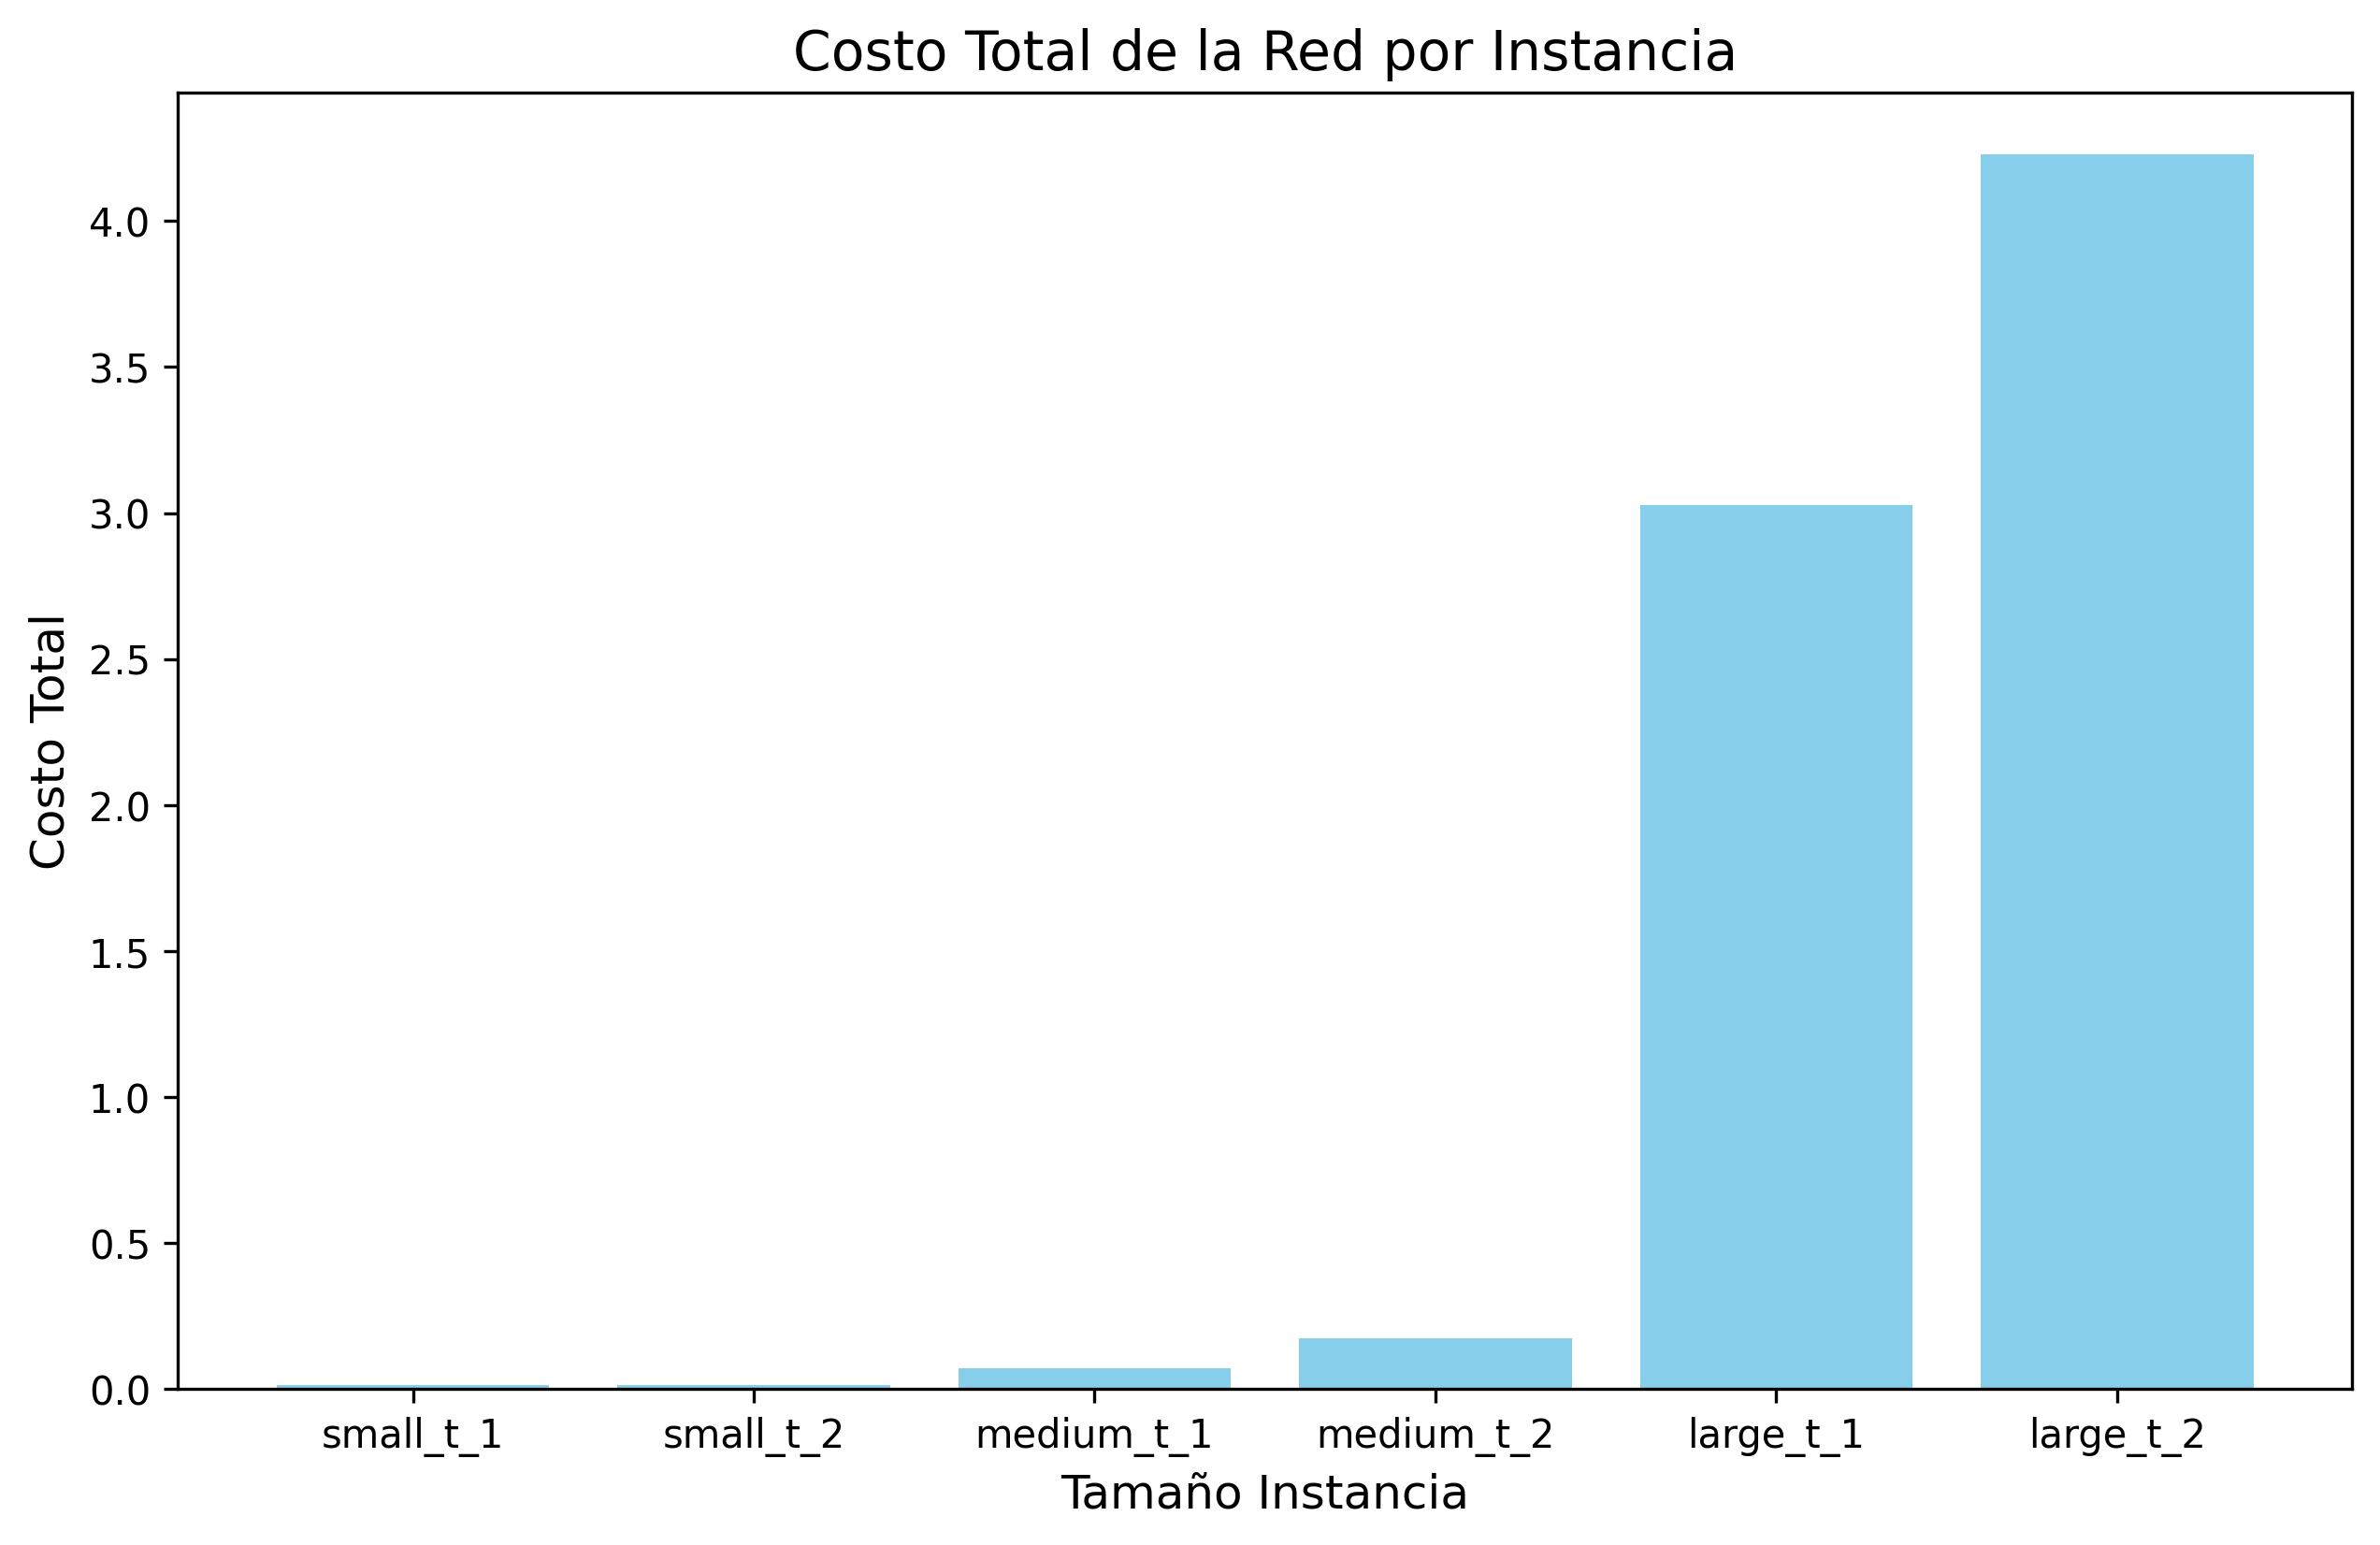
\includegraphics[width=0.8\textwidth]{time_values.png}
    \caption{Comportamiento del Tiempo de Resolución vs. Tamaño de la Instancia}
    \label{fig:tiempo_comportamiento}
\end{figure}

\end{document}
